\documentclass{beamer}

\usepackage{predavanja}
\usepackage{graphicx}
\usepackage{amsmath}
\usepackage{amsthm}
\usepackage{amssymb}
\usepackage{tikz}
\usepackage{array}
\usetikzlibrary{intersections}

{\theoremstyle{plain}
\newtheorem{izrek}{Izrek}
}

\title{Matematični izrazi in uporaba paketa \texttt{beamer}}
\subtitle{Vaje pri predmetu \emph{Računalniški praktikum}}
\institute{Fakulteta za matematiko in fiziko}
\date{}

\begin{document}

\titlepage

\begin{frame}
    \frametitle{Kratek pregled}
    \tableofcontents
\end{frame}

\section{Paket \texttt{beamer}}
\begin{frame}{Posebnosti prosojnic}
	Za prosojnice je značilna uporaba okolja \texttt{frame}, s katerim definiramo posamezno prosojnico,
	\pause
	postopno odkrivanje prosojnic,
	\pause
	ter nekateri drugi ukazi, ki jih najdemo v paketu \texttt{beamer}.
	\pause
	\begin{exampleblock}{Primer}
		Verjetno ste že opazili, da za naslovno prosojnico niste uporabili ukaza \texttt{maketitle}, ampak ukaz \texttt{titlepage}.
	\end{exampleblock}
\end{frame}

\begin{frame}{Poudarjeni bloki}
	\begin{exampleblock}{Opomba}
		Okolja za poudarjene bloke so \texttt{block}, \texttt{exampleblock} in \texttt{alertblock}.
	\end{exampleblock}
	\begin{alertblock}{Pozor!}
		Začetek poudarjenega bloka (ukaz \texttt{begin}) vedno sprejme dva argumenta: okolje in naslov bloka. Drugi argument (za naslov) je lahko prazen. 
	\end{alertblock}
\end{frame}

\begin{frame}{Tudi v predstavitvah lahko pišemo izreke in dokaze}
	\begin{izrek}
	   Praštevil je neskončno mnogo.
	\end{izrek}
	\begin{proof}
	   Denimo, da je praštevil končno mnogo.
	   \begin{itemize}[<+->]
		  \item Naj bo \(p\) \alert<4->{največje} praštevilo.
		  \item Naj bo \(q\) produkt števil \(1\), \(2\), \ldots, \(p\).
		  \item Število \(q+1\) ni deljivo z nobenim praštevilom, torej je \(q+1\) praštevilo.
		  \item To je protislovje, saj je \(q+1>p\). \qedhere
	   \end{itemize}
	\end{proof}
 \end{frame}
 


\section{Paketa \texttt{amsmath} in \texttt{amsfonts}}
\begin{frame}{Postopno odkrivanje v okolju align}
	Dokaži \emph{binomsko formulo}: za vsaki realni števili \(a\) in \(b\) in za vsako naravno število \(n\) velja
	\begin{align*}
	(a+b)^n \only<1>{ &= \ldots \\}
	\onslide<2,3>{&= (a+b) (a+b) \dots (a+b) \\}
	\onslide<3>{&= a^n + n a^{n-1} b + \dots + \binom{n}{k} a^{n-k} b^k + \dots + n a b^{n-1} + b^n \\}
	&= \sum_{k=0}^n \binom{n}{k} a^{n-k} b^k
	\end{align*}
\end{frame}


\section{Stolpci in slike}
\begin{frame}{Konstrukcija pravokotnice}
	\begin{columns}
		\begin{column}{0.5\textwidth}
			\begin{itemize}[<+->]
				\item Dana sta premica \(p\) in točka \(T\).
				\item Nariši lok \(k\) s središčem v \(T\).
				\item Lok \(k\) seče premico \(p\) v točkah \(A\) in \(B\).
				\item Nariši lok \(m\) s središčem v \(A\).
				\item Nariši lok \(n\) s središčem v \(B\) in z enakim polmerom.
				\item Loka se sečeta v točki \(C\).
				\item Premica \(TC\) je pravokotna na \(p\).
			\end{itemize}
		\end{column}
		\begin{column}{0.5\textwidth}
			\only<1>{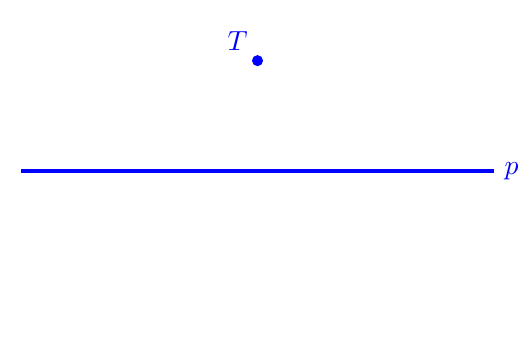
\includegraphics[width=50mm]{slike/fig-1.png}}
			\only<2>{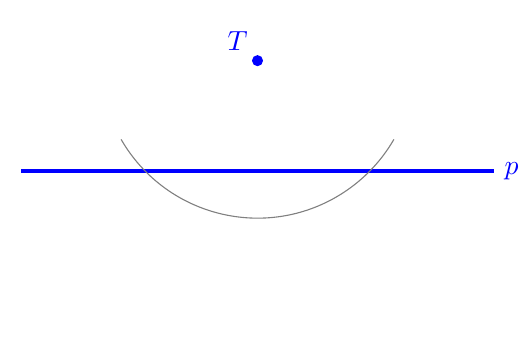
\includegraphics[width=50mm]{slike/fig-2.png}}
			\only<3>{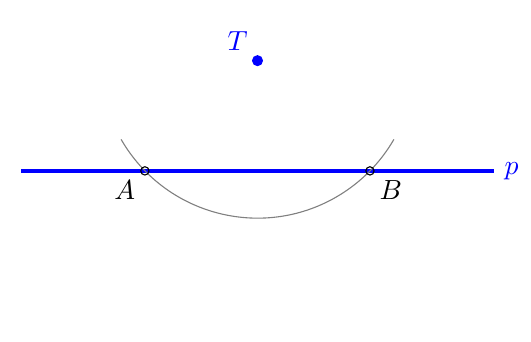
\includegraphics[width=50mm]{slike/fig-3.png}}
			\only<4>{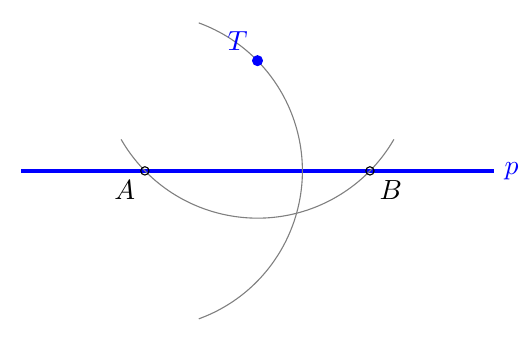
\includegraphics[width=50mm]{slike/fig-4.png}}
			\only<5>{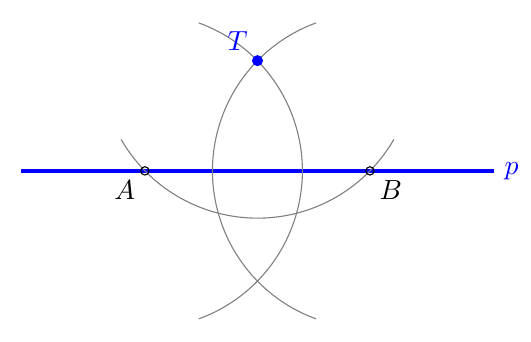
\includegraphics[width=50mm]{slike/fig-5.png}}
			\only<6>{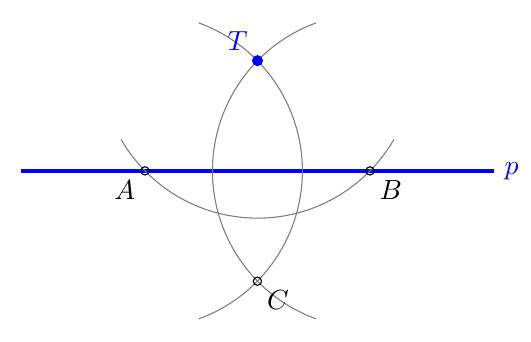
\includegraphics[width=50mm]{slike/fig-6.png}}
			\only<7>{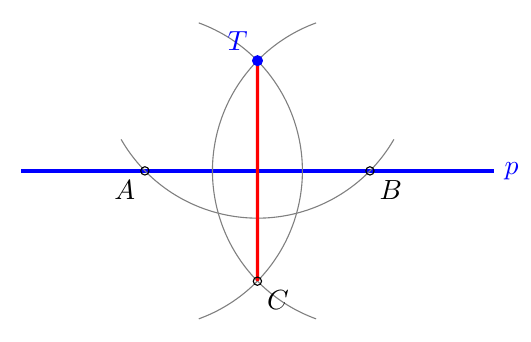
\includegraphics[width=50mm]{slike/fig-7.png}}
		\end{column}
	\end{columns}
			
\end{frame}


\section{Paket \texttt{beamer} in tabele}
\begin{frame}{Odkrivanje tabele po vrsticah}
	Včasih pride prav, da tabelo odkrivamo postopoma po vrsticah.
	\begin{center}
		\begin{tabular}{c|cccc}
		   Oznaka & A & B & C & D \\ \hline
		   \onslide<2->{X & 1 & 2 & 3 & 4 \\}
		   \onslide<3->{Y & 3 & 4 & 5 & 6 \\}
		   \onslide<4->{Z & 5 & 6 & 7 & 8}
		\end{tabular}
	\end{center}
\end{frame}
 

\begin{frame}{Odkrivanje tabele po stolpcih}
	Tabelo lahko odkrivamo tudi po stolpcih, čeprav ni najlažje.

	\begin{center}
		\begin{tabular}{c|cccc}
		   Oznaka & \onslide<2->{A} & \onslide<3->{B} & \onslide<4->{C} & \onslide<5->{D} \\ \hline
		   X & \onslide<2->{1} & \onslide<3->{2} & \onslide<4->{3} & \onslide<5->{4} \\
		   Y & \onslide<2->{3} & \onslide<3->{4} & \onslide<4->{5} & \onslide<5->{6} \\
		   Z & \onslide<2->{5} & \onslide<3->{6} & \onslide<4->{7} & \onslide<5->{8}
		\end{tabular}
	\end{center}
\end{frame}


\section{Risanje s paketom TikZ}
\begin{frame}{Konstrukcija pravokotnice}
	\centering
	\begin{tikzpicture}
		\coordinate (T) at (0, 1.4);
		\onslide<1->{\draw[blue, very thick, name path=p] (-3, 0) -- (3, 0) node[right] {$p$};}
		\onslide<2->{\draw[gray, name path=k] (T) ++(210:2) arc (210:330:2);}
		\onslide<2->{\path[name intersections={of=p and k, by={A, B}}];}
		\onslide<3->{\draw[gray, name path=m] (A) ++(-70:2) arc (-70:70:2);}
		\onslide<4->{\draw[gray, name path=n] (B) ++(250:2) arc (250:110:2);}
		\onslide<5->{\path[name intersections={of=m and n, by={C, T'}}];}
		\onslide<6->{\draw[red, very thick] (T) -- (C);}
		\onslide<1->{\fill[blue] (T) circle (2pt) node[above left] {$T$};}
		\onslide<2->{\draw (A) circle (1.5pt) node[below left] {$A$};}
		\onslide<2->{\draw (B) circle (1.5pt) node[below right] {$B$};}
		\onslide<5->{\draw (C) circle (1.5pt) node[below right] {$C$};}
	\end{tikzpicture}
\end{frame}

\end{document}